\section{The NEXT Infrastructures}
\label{sec.infra}
%%%%%%%%%%


Figure \ref{fig:F6:F6} shows the layout of the experimental area. All the system is deployed on a working platform, made of Tramex of $11 \times 11 \mathrm{m^2}$~shown in figure \ref{fig:F2:F2}. The NEW detector is hosted inside a lead castle (figure \ref{fig:F4:F4}) and sitting in a seismic platform (figure \ref{fig:seismicPedestal3D}). 
The seismic pedestal is frame with rectangular beams and 8 isolator seismic blocks. The pedestal is designed to swing without breaking in the event of earthquakes one order of magnitude larger than the maximum earthquake recorded in Canfranc. 

The lead castle is made of lead blocks placed into a steel frame. The blocks are organised in a staggered structure to maximise the amount of lead seen by the external radiation. Additional steel sheets (made of radiopure steel-Ti alloy) provide the needed rigidity to avoid creep. The total weight of the lead is about 58 tons. 

The platform and seismic pedestal were built in 2014. The leas castle has been completed in 2015.


\begin{figure}[hpt!]
    \bigskip
    \begin{center}\leavevmode
        \rotatebox{0}{
        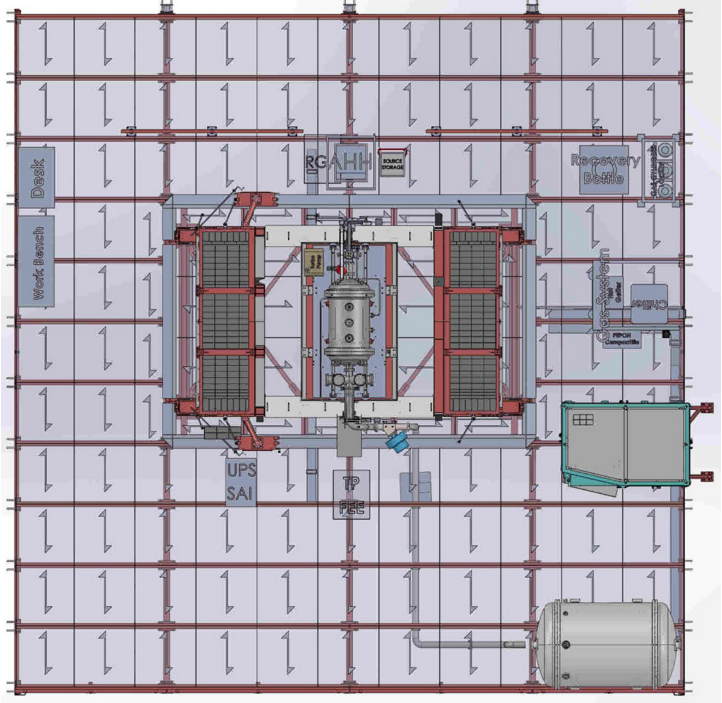
\includegraphics[width=\textwidth, ]{GasSystemAndInfrastructures/IMG/F6.png}}
        \caption{\textit{Layout of the NEXT working platform.}}
        \label{fig:F6:F6}
    \end{center}
\end{figure}

\begin{figure}[hpt!]
    \bigskip
    \begin{center}\leavevmode
        \rotatebox{0}{
        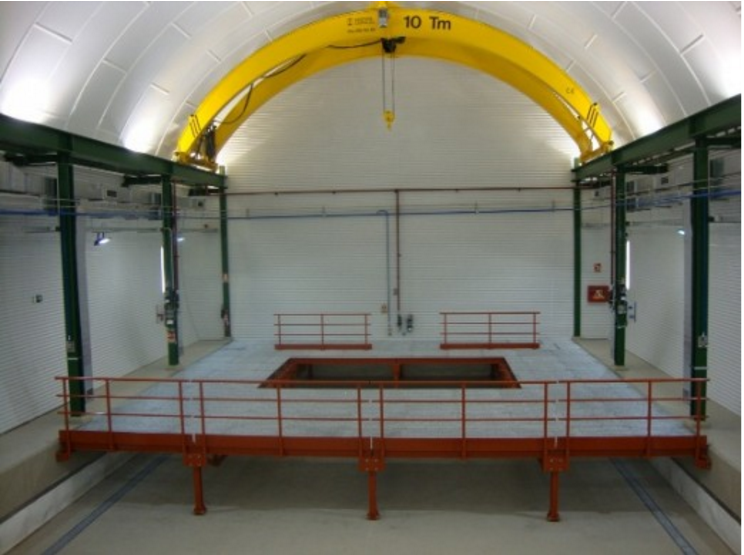
\includegraphics[width=\textwidth, ]{GasSystemAndInfrastructures/IMG/F2.png}}
        \caption{\textit{The NEXT working platform, empty}}
        \label{fig:F2:F2}
    \end{center}
\end{figure}

\begin{figure}[hpt!]
    \bigskip
    \begin{center}\leavevmode
        \rotatebox{0}{
        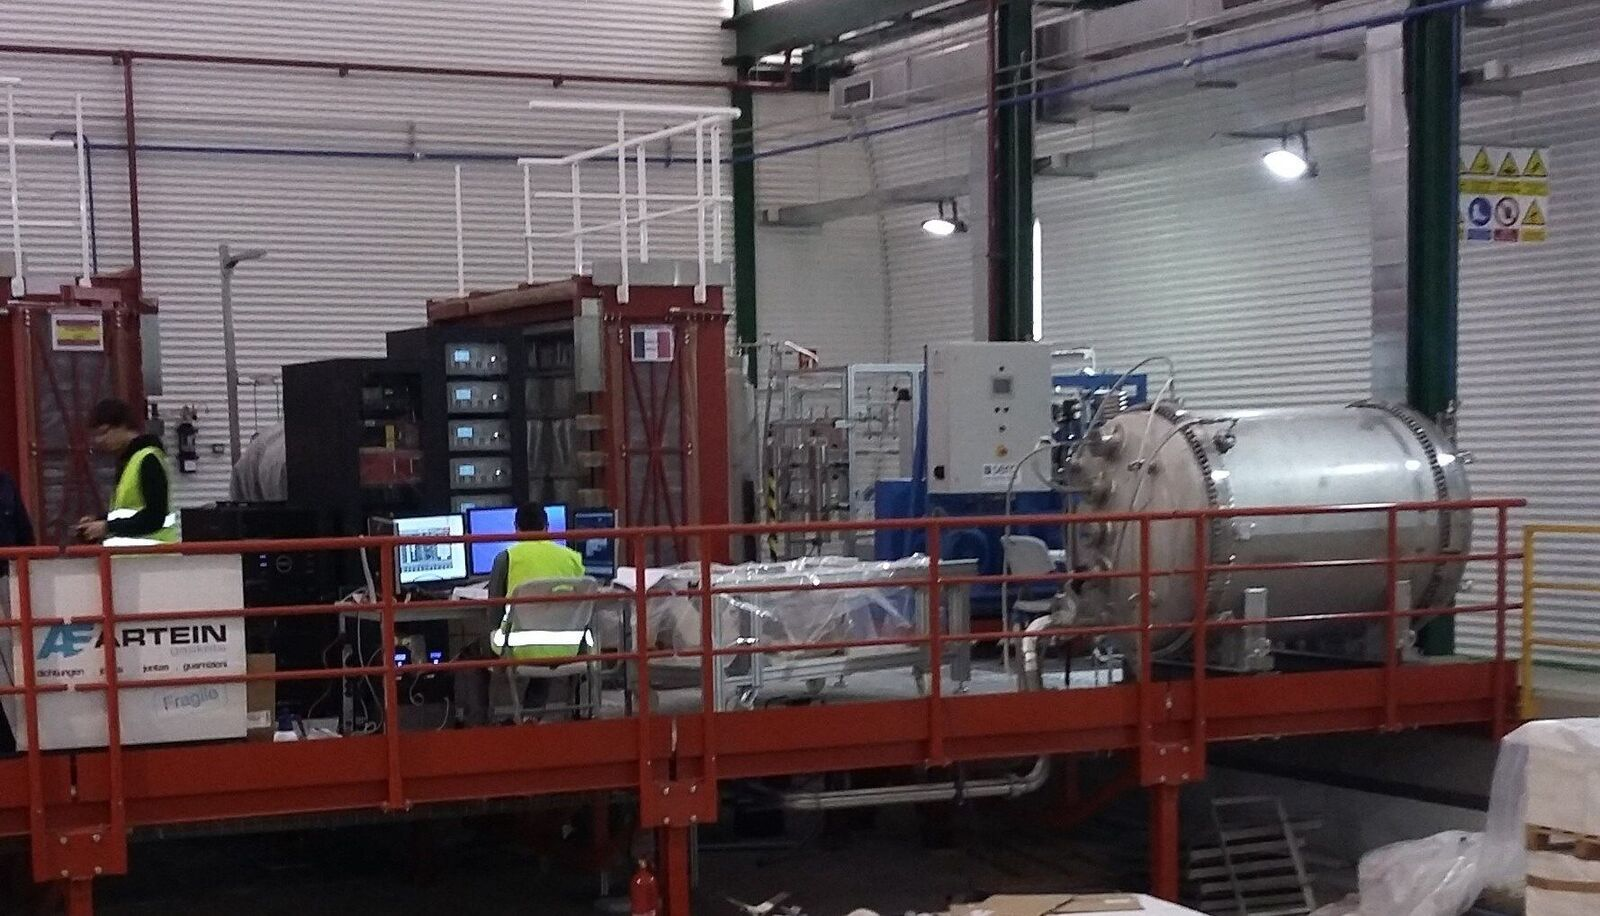
\includegraphics[width=\textwidth, ]{img/Platform1.jpg}}
        \caption{\textit{The NEXT working platform, with infrastructures installed}}
        \label{fig:F2:F2}
    \end{center}
\end{figure}



\begin{figure}[hpt!]
    \bigskip
    \begin{center}\leavevmode
        \rotatebox{0}{
        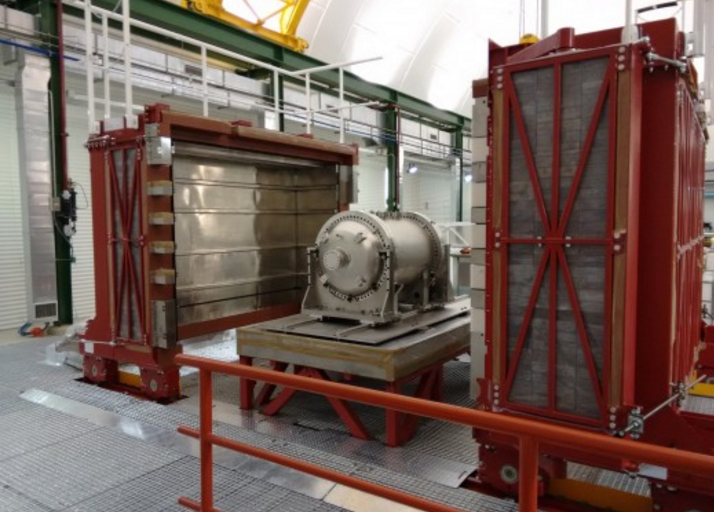
\includegraphics[width=\textwidth, ]{GasSystemAndInfrastructures/IMG/F4.png}}
        \caption{\textit{The lead castle in open position}}
        \label{fig:F4:F4}
    \end{center}
\end{figure}

\begin{figure}[hpt!]
\centering
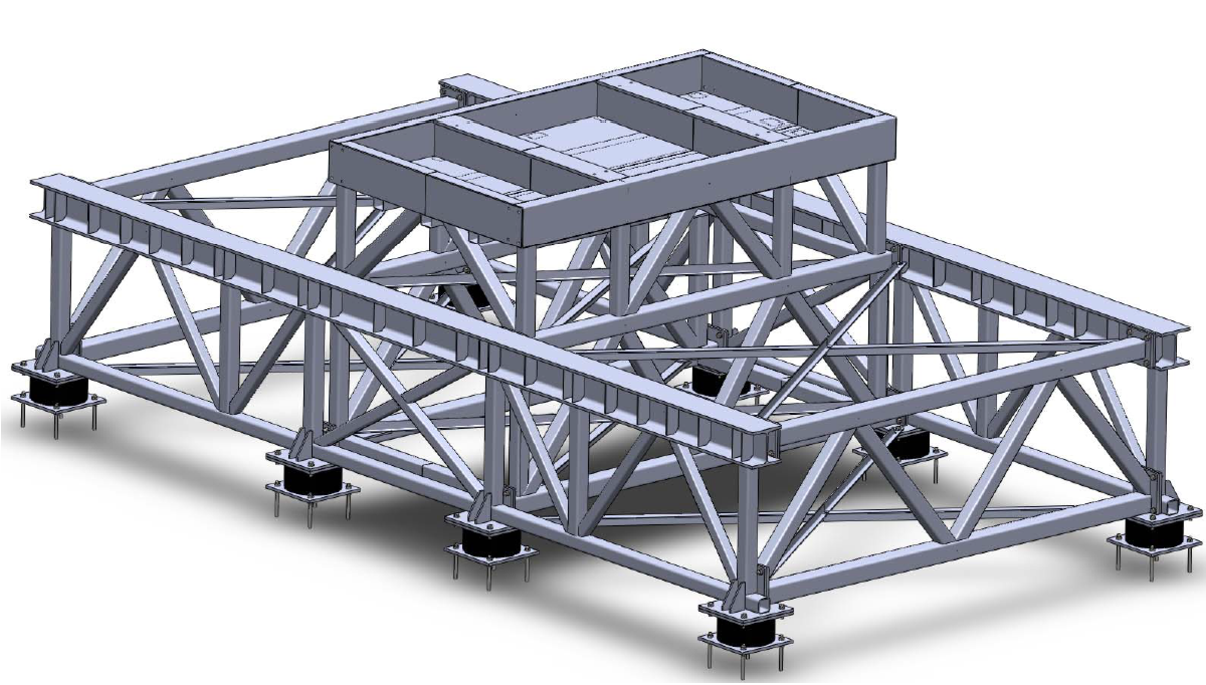
\includegraphics[height=8cm]{img/SeismicPedestal.pdf}
\caption{A 3D view of the Seismic Pedestal (SP).} \label{fig:seismicPedestal3D}
\end{figure}



%\begin{figure}
%\centering
%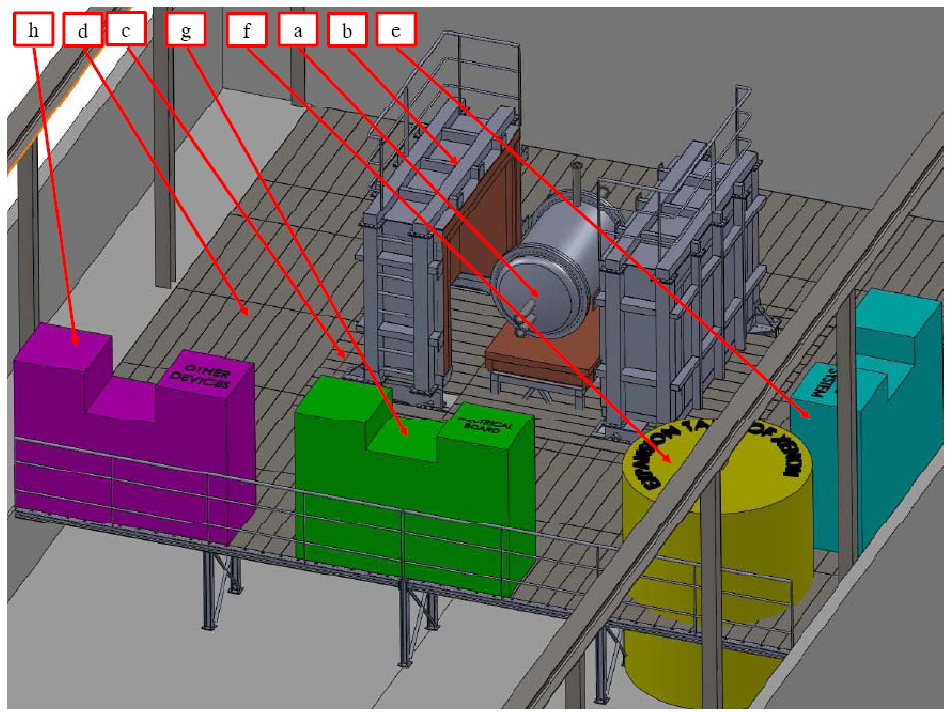
\includegraphics[height=12cm]{img/InfraStruc.pdf}
%\caption{The NEXT infrastructures: (a) The pressure vessel, hosting the detector; (b) the lead castle shield in its open configuration; (c) seismic platform; (d) working platform; (e) gas purification system; (f) emergency gas vent tank; (g) data acquisition system; (h) other systems.} \label{fig:Infrastructure}
%\end{figure}
%
%\begin{figure}
%\centering
%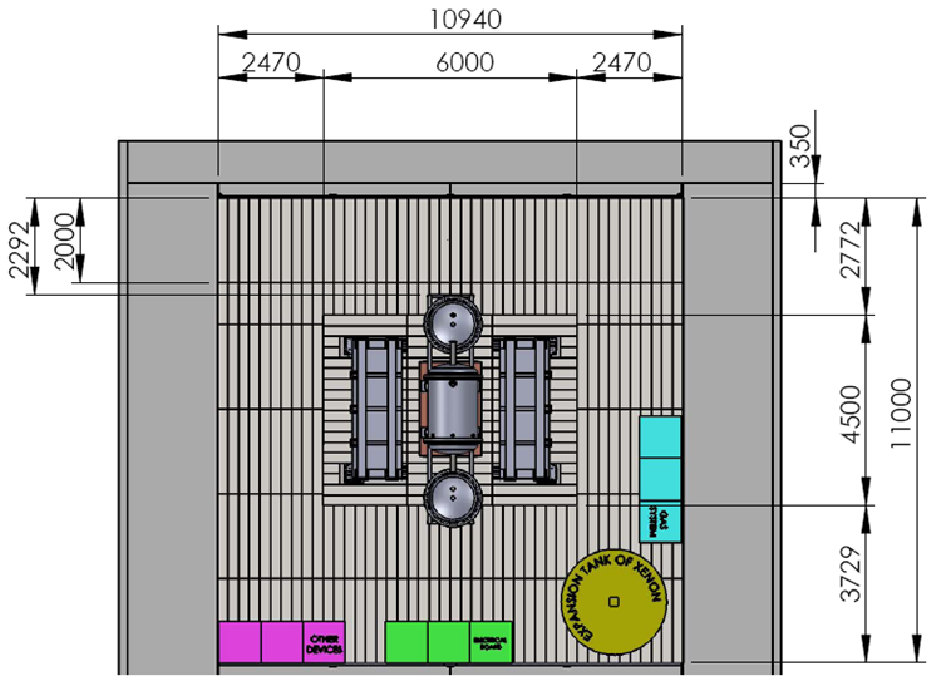
\includegraphics[height=12cm]{img/InfraStruc_2.pdf}
%\caption{The NEXT-100 infrastructures (top view) showing the overall dimensions of the installation.} \label{fig:Infra2}
%\end{figure}


\subsection*{The gas system}



\begin{figure}[hpt!]
    \bigskip
    \begin{center}\leavevmode
        \rotatebox{0}{
        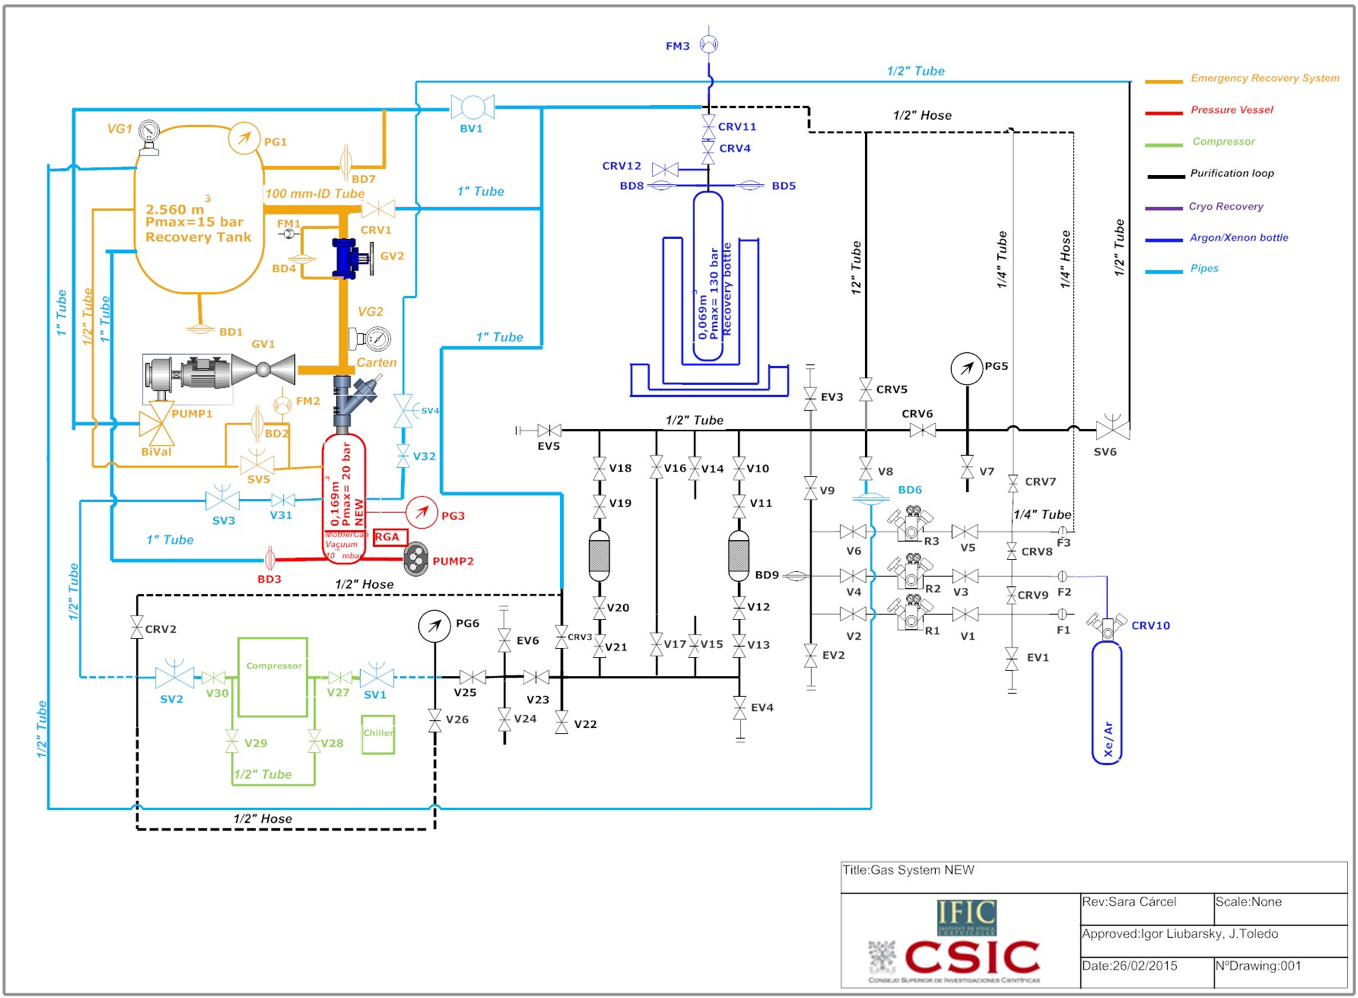
\includegraphics[width=\textwidth, ]{img/Gas1.png}}
        \caption{\textit{A functional schema of the NEXT Gas System}}
        \label{fig:F8:F8}
    \end{center}
\end{figure}

Xenon circulates through the detector via a gas recirculation and purification system (figure \ref{fig:F8:F8}).


The goal of the gas system (GS) is to purify the xenon gas used by the NEXT detectors, reducing the traces of gases such as ${\rm O, CO_2,CO, H_2, N_2, CH_4}$~ and water vapour to less than one part per billion (ppb). Both NEW and NEXT-100 will operate with natural xenon (NXe) and enriched xenon (EXe). The gas will be maintained at room temperature and 10--15 bar pressure inside the detector(s). The gas system has been designed to avoid significant losses of xenon under all foreseeable circumstances.

\begin{figure}[hpt!]
    \bigskip
    \begin{center}\leavevmode
        \rotatebox{0}{
        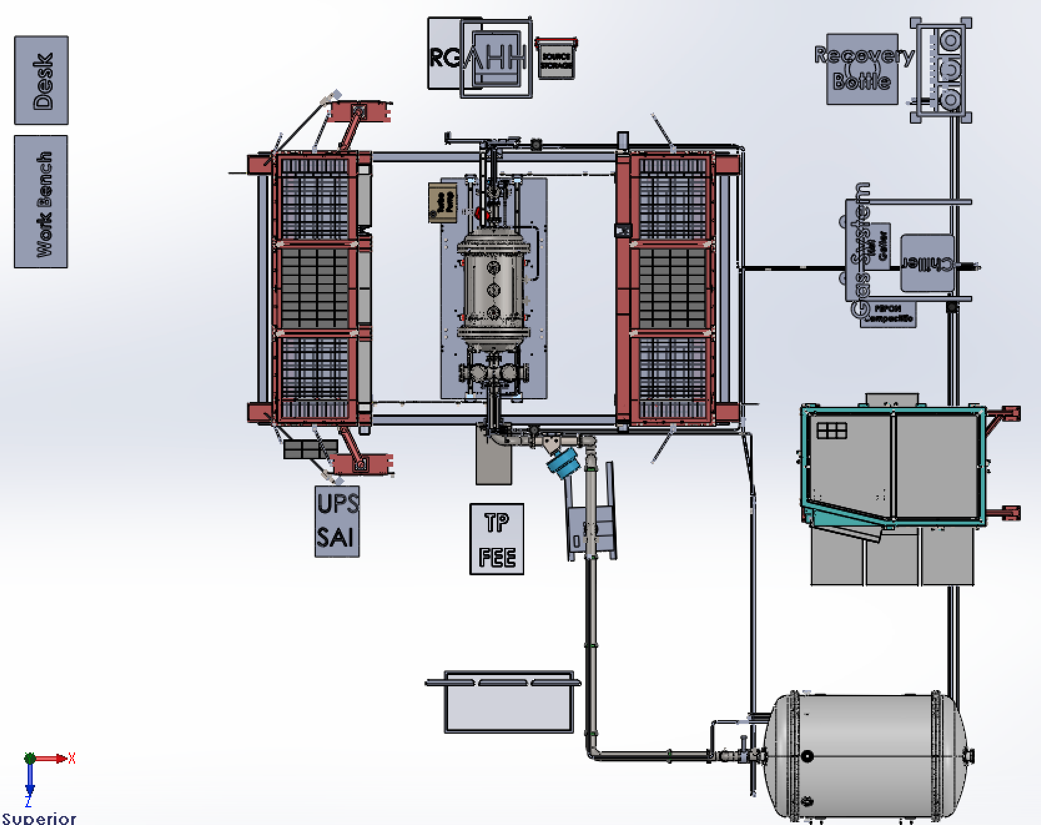
\includegraphics[width=\textwidth, ]{img/Gas2.png}}
        \caption{\textit{Drawing showing the main components of the NEXT gas sytem.}}
        \label{fig.gas2}
    \end{center}
\end{figure}

Figure \ref{fig:F8:F8} shows a schematics of the gas system. Its main components (figure \ref{fig.gas2}) are:  

\begin{itemize}
\item Emergency recovery system.
\item Pressure vessel (NEW or NEXT-100). 
\item Compressor.
\item Purification loop.
\item Cryo-recovery.
\item Argon/xenon bottles.
\item Pipes.
\item Control System.
\end{itemize}

The pipes are all plumed together using ?? and 1? stainless tube and flexible hoses where mechanical insulation is required. The total amount of gas in the supply bottle and also in the system will be such that in the event of the entire bottle emptying into the system and being vented into the emergency recovery tank the final pressure will not exceed 3 bar.

\subsubsection*{Emergency recovery tank and ancillary systems}

\begin{figure}[hpt!]
    \bigskip
    \begin{center}\leavevmode
        \rotatebox{0}{
        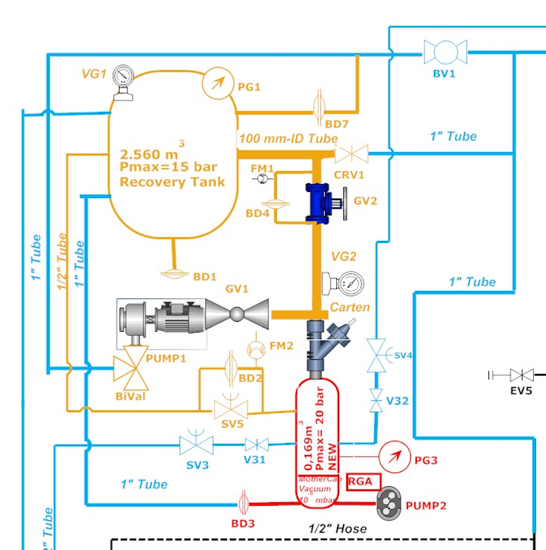
\includegraphics[width=\textwidth, ]{img/GasER.png}}
        \caption{\textit{Emergency Recovery part of the Gas System}}
        \label{fig.GER}
    \end{center}
\end{figure}

\begin{figure}[hpt!]
    \bigskip
    \begin{center}\leavevmode
        \rotatebox{0}{
        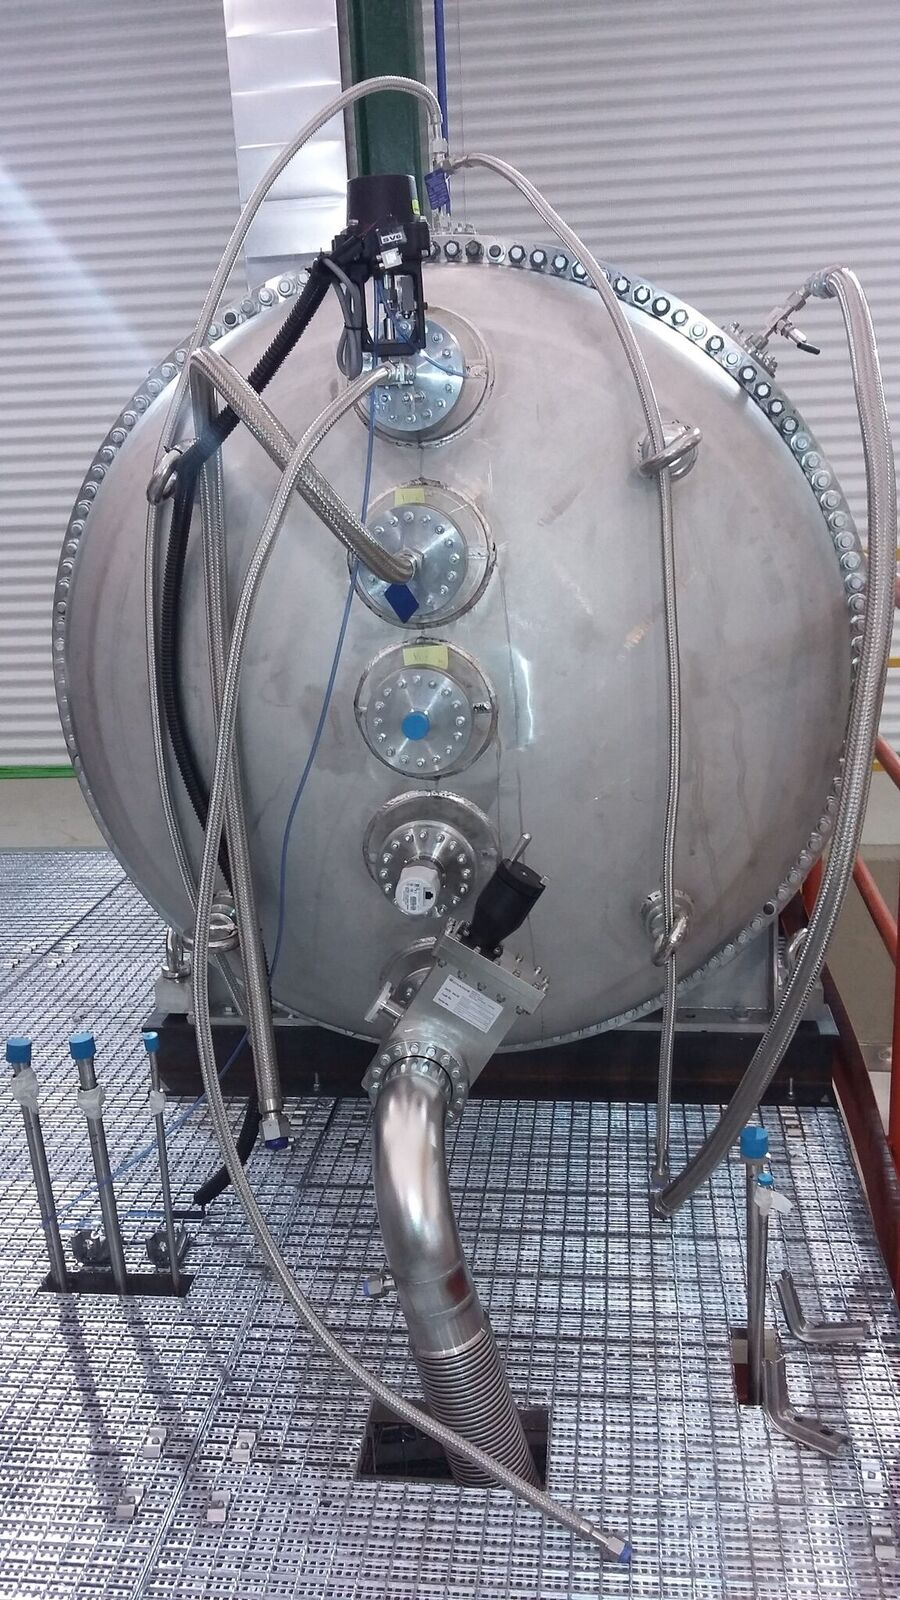
\includegraphics[width=10cm ]{img/NEXT100AsRecoveryVessel.jpg}}
        \caption{\textit{The NEXT-100 pressure vessel operating as Emergency Recovery Tank.}}
        \label{fig.N100}
    \end{center}
\end{figure}

\begin{figure}[hpt!]
    \bigskip
    \begin{center}\leavevmode
        \rotatebox{0}{
        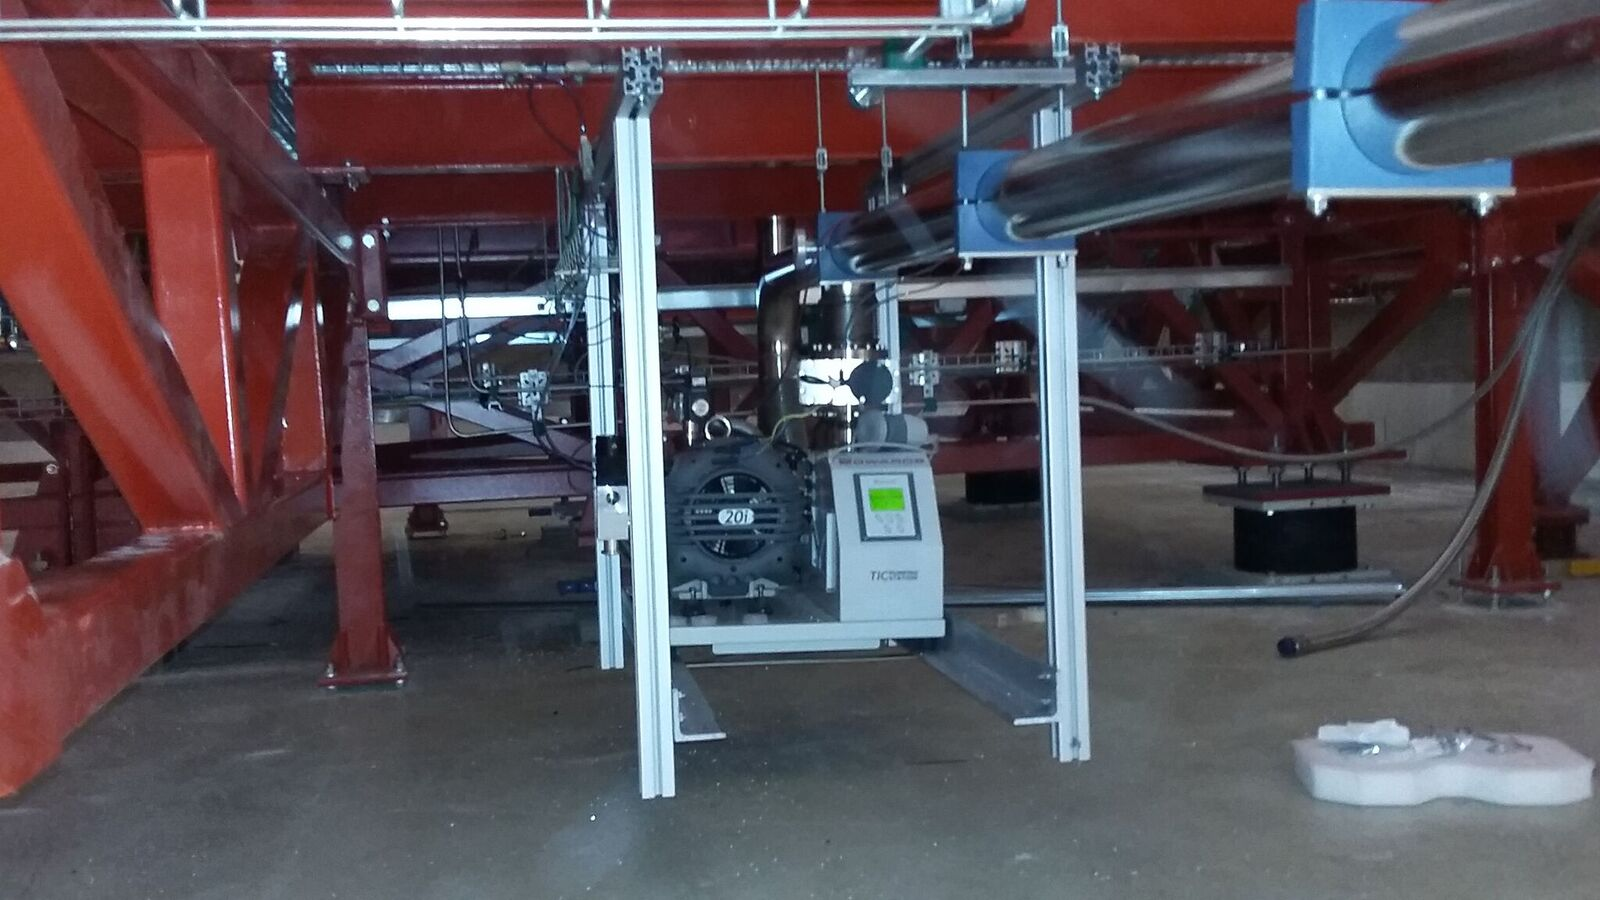
\includegraphics[width=\textwidth, ]{img/PUMP1.jpg}}
        \caption{\textit{A picture of the vacuum pump (PUMP1) used to keep the recovery tank at a 
        nominal pressure of $10^{-5}$~mbar. The pump is sitting under the working platform.}}
        \label{fig.P1}
    \end{center}
\end{figure}


The emergency recovery section of the gas system (figure \ref{fig.GER}) is designed to recover gas into a recovery tank in the event of over pressure in the gas system. During the operation of NEW, the existing pressure vessel of the NEXT-100 experiment (a tank with a volume of 2.560 m$^3$~ made of 316Ti alloy and with CE certification for operation at 15 bar) is reused as recovery tank (figure \ref{fig.N100}). In order to guarantee that gas is dumped into the recovery tank in the event of an over-pressure, the tank is kept during normal operations at $10^{-5}$~mbar. This is done by pumping the tank with the vacuum pump PUMP1 (figure \ref{fig.P1})
through valves GV1 (this is a pneumatic-activated guillotine valve, certified to separate pressure from vacuum zones) and the manual valve GV2 which acts as a backup. The system is backed by a third pneumatic valve, BiVal. A pressure gauge (PG1) and a vacuum gauge (VG1) measure the pressure and vacuum in the recovery tank. A bursting disk installed in the recovery tank (BD1) will burst at 5 bar, avoiding any over-pressure in the system (notice that a pressure of 5 bar in the emergency recovery tank is equivalent to a pressure of 50 bar in the NEW pressure tank which is the maximum pressure that the vessel can tolerate). 
%A second disk, BD7, will break at 3 bar. The disk function is to avoid an over pressure over 30 bar in the gas system. In practice, BD7 is relevant only in case that BV1 is opened by mistake when there is pressure in the purification loop. 

In normal operations, the vacuum pump (PUMP1) is pumping the recovery tank and GV1 is opened. The valve is automatically controlled by the Slow Control System and to be open needs a pneumatic pressure of 4.5-5 bar and a voltage of 24 VDC. This implies that the valve closes in failure (electrical of pneumatic shutdown at the experiment or the LSC). Also, if an emergency condition (need to recover the gas) arises, PUMP1 is turned off and GV1 closes. Emergency conditions are normally triggered by excess pressure in the NEW pressure vessel. In this case, the Carten Valve opens up and as GV2 is always open, the gas will evacuate to the tank through the safety evacuation line.A second pneumatic valve, SV6 is controlled by the Slow Control System and will open up in the event of excess pressure. If both the Carten valve and SV6 fail, disk BD2 will burst at 13 bar. 

\subsubsection*{Recirculation compressor}

\begin{figure}[hpt!]
\centering
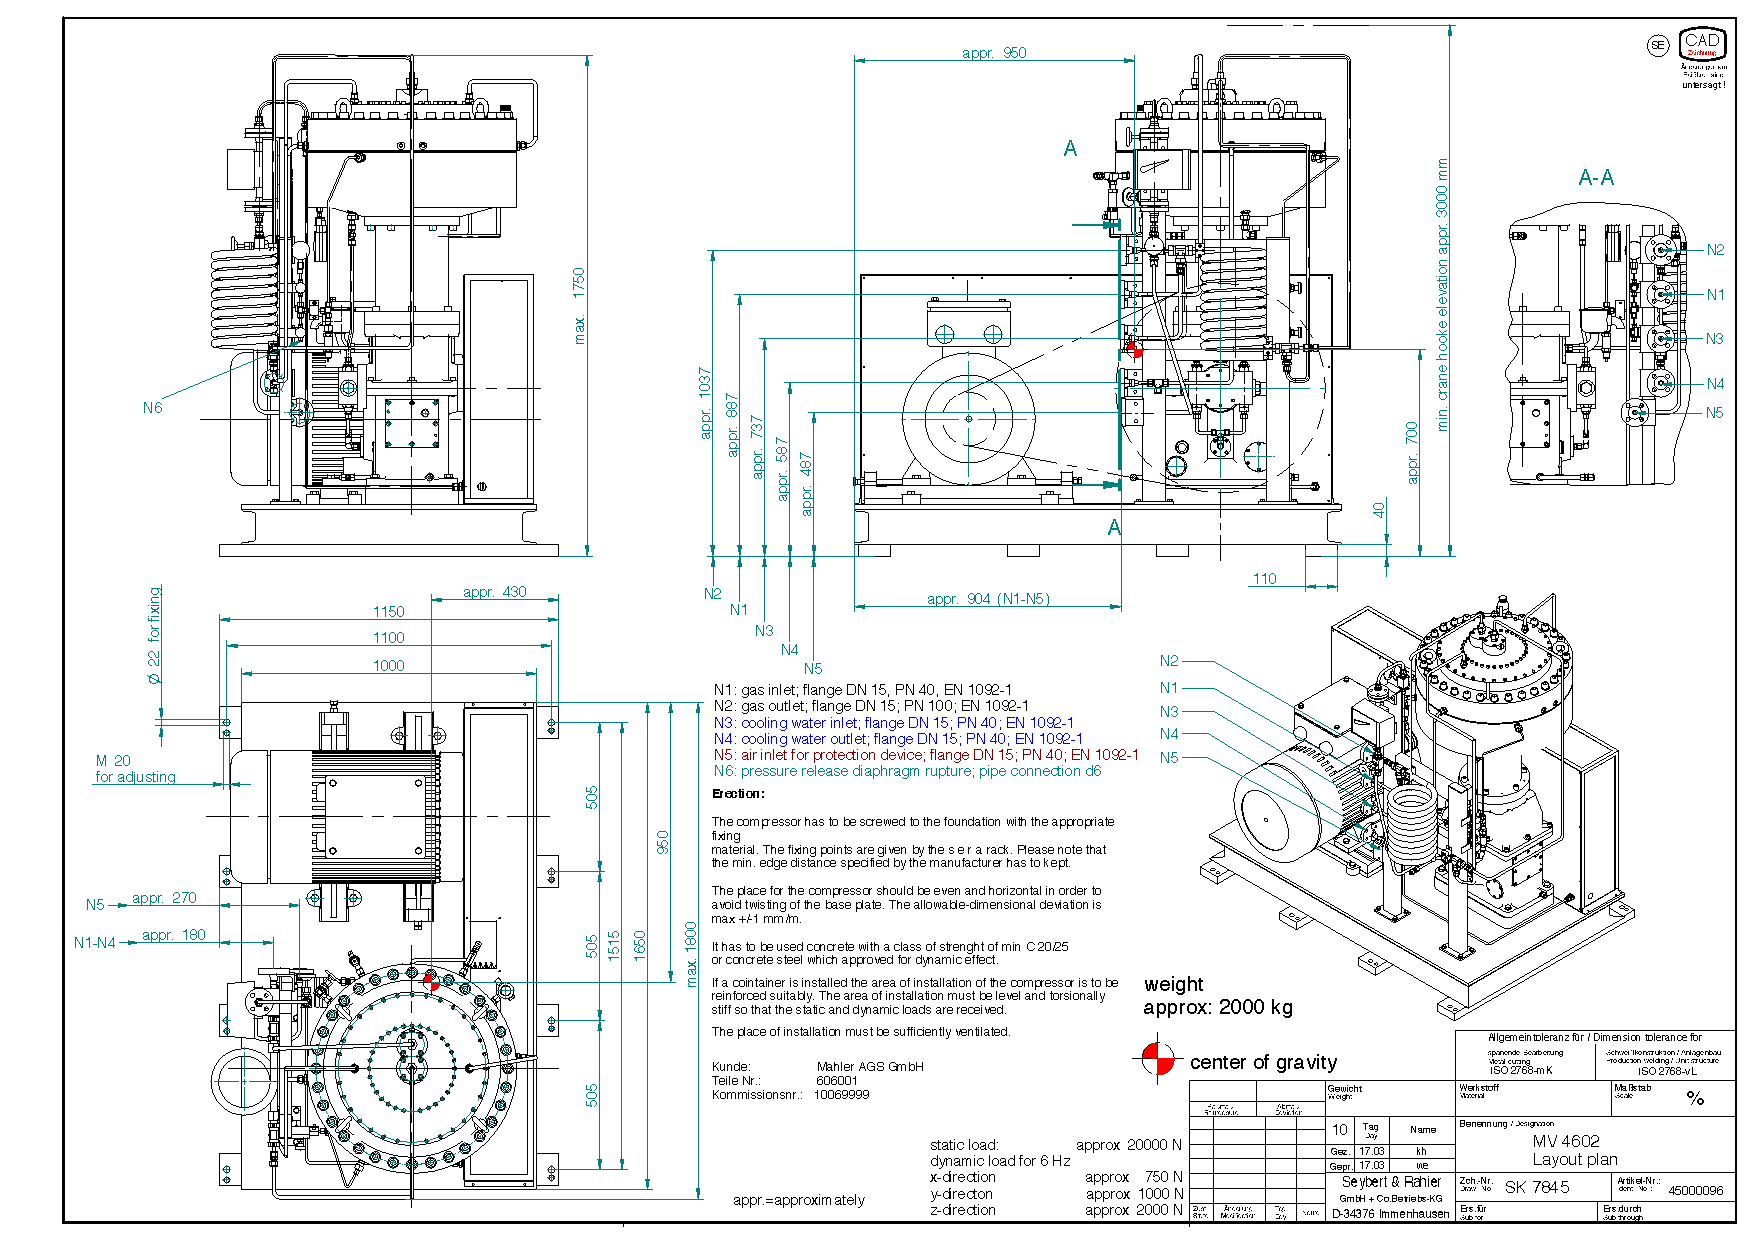
\includegraphics[height=12cm]{img/Pump.pdf}
\caption{Schematics of the SERA recirculation compressor, chosen by NEXT.} \label{fig:pump}
\end{figure}

\begin{figure}[hpt!]
\centering
\includegraphics[height=12cm]{img/Compressor2.png}
\caption{A picture of the compressor.} \label{fig.sera}
\end{figure}


The most vulnerable component of the gas system is the compressor, which acts as a re-circulation pump. The enriched xenon is very expensive and therefore the pump to move the gas through the re-circulation loop must have sufficient redundancy to minimise the probability of failure and leakage. Furthermore, to preserve the purity of the gas all metal to metal seals must be used. 

Figure \ref{fig:pump} shows the schematics of the compressor chosen for NEXT, manufactured by the SERA company, in Germany. The pump is made with metal-to-metal seals on all the wetted surfaces. The gas is moved through the system by a triple stainless steel diaphragm. Between each of the diaphragms there is a sniffer port to monitor for gas leakages. In the event of a leakage automatic emergency shutdown can be initiated. Figure \ref{fig.sera} shows a picture of the compressor, already installed at the LSC. 

\subsubsection*{Hot getter}

\begin{figure}[hpt!]
\centering
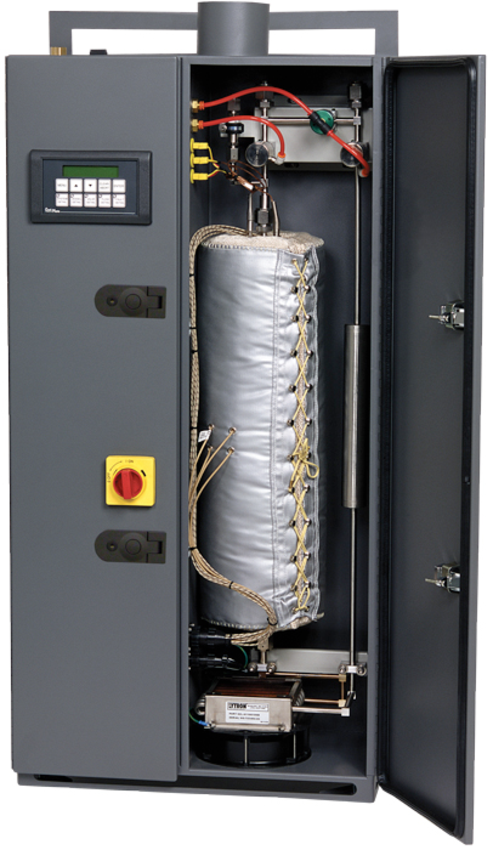
\includegraphics[height=10cm]{img/Getter.pdf}
\caption{The PS4-MT50 SAES hot getter chosen to purify the gas.} \label{fig:getter}
\end{figure}

SAES PS4-MT50 hot getter (figure \ref{fig:getter}) has been chosen as the main purification filter for the xenon gas. The getter is capable of removing electron negative impurities to less than 1 ppb and deploys a nominal flow rate of 150 slpm, offering sufficient spare capacity. The gas system will contain two such getters in parallel with a bypass. The advantage of hot getter technology
is their capability to remove nitrogen and methane (in addition to oxygen, water and carbon dioxide). Furthermore, hot getters are known to emit less radon than cold getters.  

\subsubsection*{Recirculation loop and cryo-recovery }

\begin{figure}[hpt!]
\centering
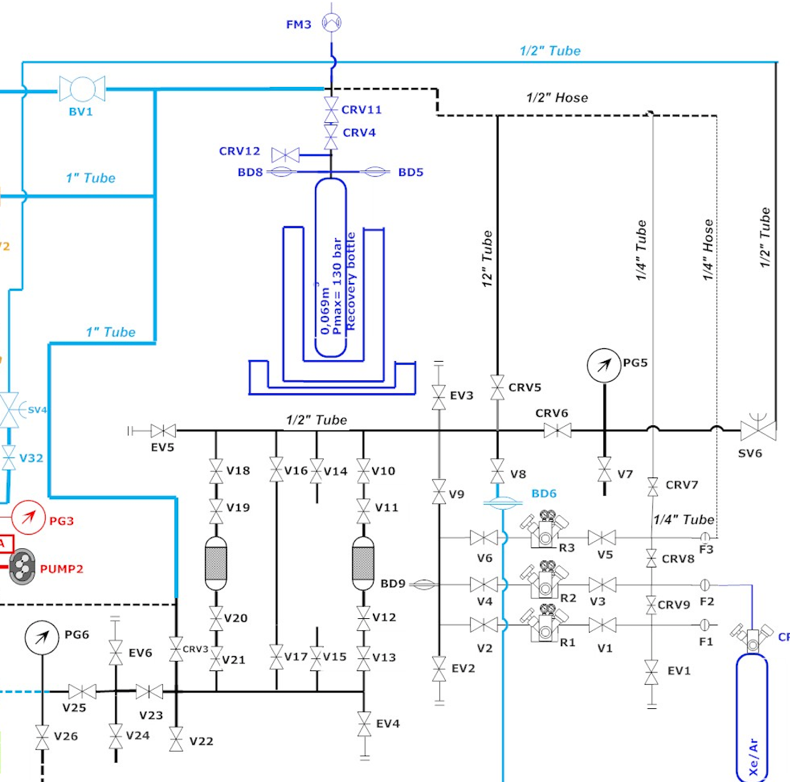
\includegraphics[height=12cm]{img/Recirculation.png}
\caption{An scheme of the recirculation loop and cryo-recovery part of the gas system.} \label{fig:ct}
\end{figure}

Figure \ref{fig.ct} shows the recirculation loop. The gas enter the system from the pressure bottles, through a regulator and circulates through cold and/or hot getters. To recover the gas in normal conditions we use a permanently chamber cooled by liquid Nitrogen (cryo-recovery or CR), also shown in figure \ref{fig.ct}. 

\subsubsection*{Summary}
 
The needed infrastructures for the NEXT experiment have been completed during 2015 and the first quarter of 2016. The gas system is now in the final commissioning phase, and ready to pass the tests needed for underground operation certification. 
